\section{Analysis Strategy}\label{sec:ggtt_analysis strategy}

Events are selected beginning with one of two different diphoton triggers, one which requires $\mgg > 90$\GeV, and another than requires $\mgg > 65$\GeV but has a reduced luminosity of 132\fbinv. The former is used for all searches except for the \XYggHtt search when $\mY<125$\GeV. The \XYggHtt search is therefore treated as two different searches, a \textit{low-mass} search for $\mY < 125$\GeV and a \textit{high-mass} search for $\mY > 125$\GeV. Following the trigger, preselection criteria are applied which includes the requirement of at least one tau lepton candidate, and a selection on \mgg which corresponds to 100--180\GeV for the \XHH and \XYttHgg searches, while in the low and high-mass \XYggHtt searches, it corresponds to 65--150\GeV and 100--1000\GeV respectively. The triggering and preselection requirements are described in greater detail in \cref{sec:ggtt_trigger_preselection}. 

Toy examples of the \mgg distributions for the signal and background processes for each search are shown in \cref{fig:toy_examples}. In every search, there is a nonresonant background which is predominantly comprised of prompt photon and diphoton production with associated jets (\gjet and \ggjet), where the jets are misidentified as photons and/or tau leptons. There are also smaller contributions from \vgamma, \ttbar, \ttgamma, and \ttgammagamma where the vector bosons (from direct production or the decay of top quarks) can decay into tau leptons and associated jets can be misidentified as photons. This nonresonant background forms a smoothly-falling distribution in \mgg. 

Furthermore, there is a resonant background in every search from single Higgs boson production in the SM, where the Higgs boson decays to two photons. This background leads to a peak in the \mgg distribution at the Higgs boson mass ($\approx125\GeV$). In the low-mass \XYggHtt search, there is another resonant background present at about 91\GeV from \Zee decays where both electrons are misidentified as photons. This background is referred to as the DY background since it predominantly comes from the Drell-Yan (DY) process.

The signal process forms a peak in the \mgg distribution at a location depending on the search and \mY. In the \XHH and \XYttHgg searches, the two photons originate from a Higgs boson and therefore form a peak at about 125\GeV. In the \XYggHtt searches, the photons originate from the $\PY$ scalar and therefore form a peak at \mY. 

\begin{figure}
  \centering
  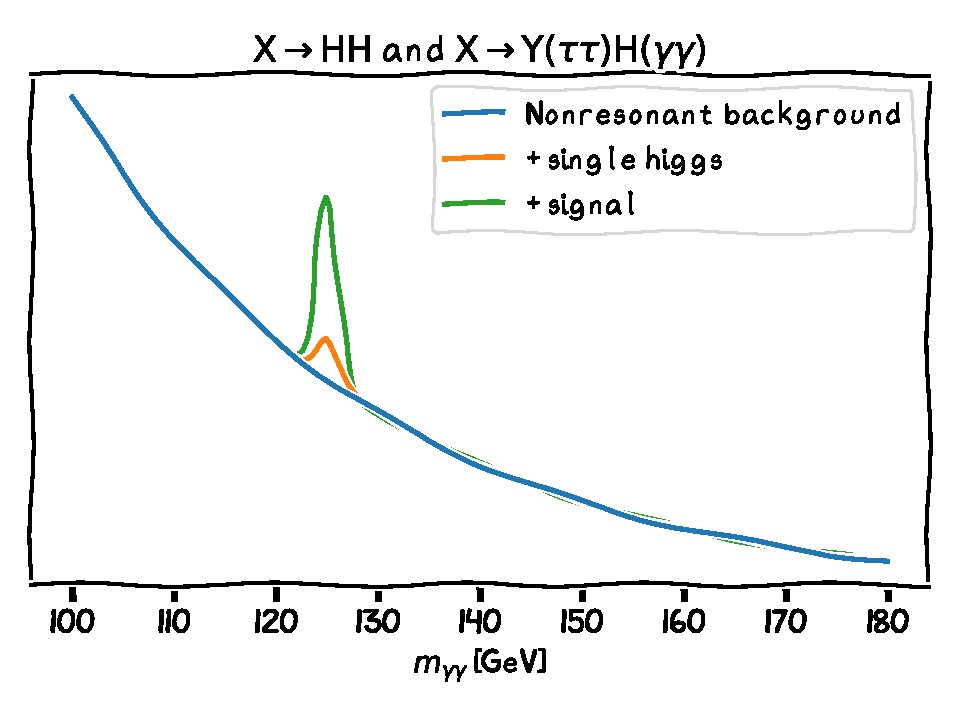
\includegraphics[width=0.49\textwidth]{Figures/Dihiggs/introduction/xhh.pdf}\\
  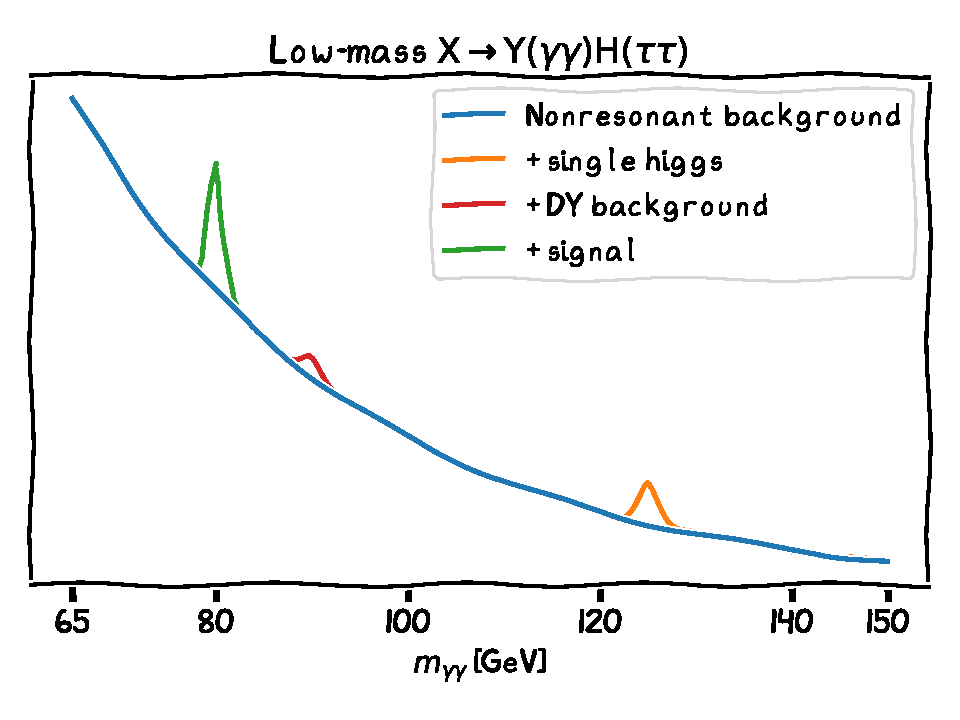
\includegraphics[width=0.49\textwidth]{Figures/Dihiggs/introduction/xyh_low_mass.pdf}
  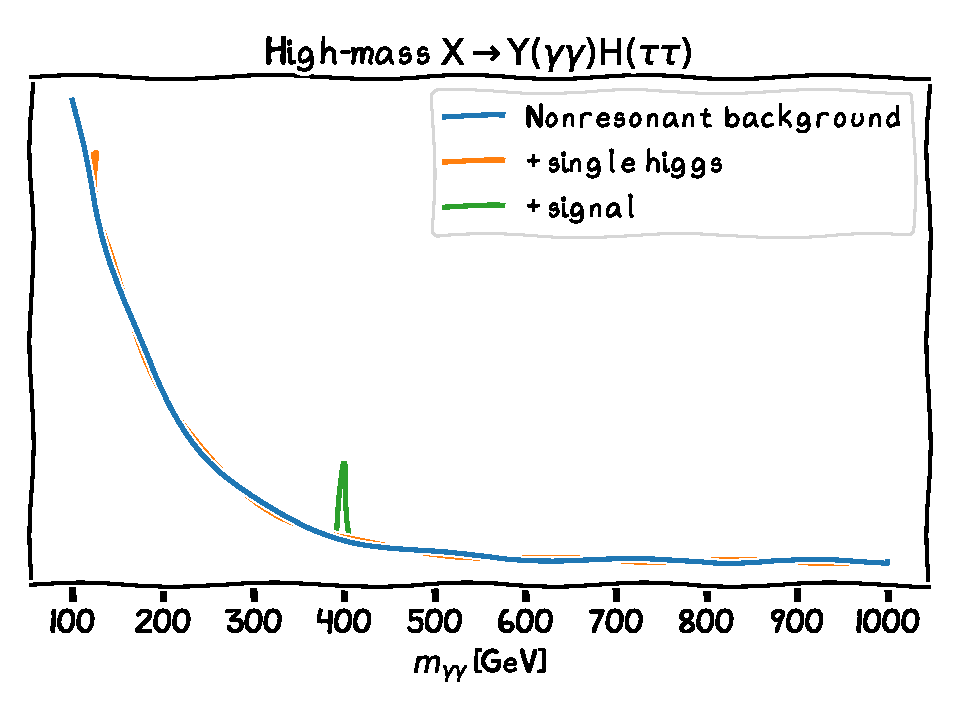
\includegraphics[width=0.49\textwidth]{Figures/Dihiggs/introduction/xyh_high_mass.pdf}
  \caption[Signal and Background \mgg Distributions in the Di-Higgs Search]{Toy examples of the \mgg distributions of the background and signal processes for each search. In each search, there is a smoothly-falling nonresonant background (blue), and a background from SM single Higgs production (orange). In the low-mass search, there is also a DY background (red) originating from the misidentification of electrons as photons in \Zee decays. The signal peaks at about 125\GeV in the \XHH and \XYttHgg searches, and at \mY in the \XYggHtt searches, where examples at $\mY=80$ and 400\GeV are shown for the low and high-mass searches respectively. The shape and relative rates of every process are not exact and are for illustrative purposes only.}\label{fig:toy_examples}
\end{figure}

To improve the sensitivity of the search, signal events are separated from background events using a machine learning classifier. Neural networks that are trained to be parametric in \mX, and \mY in case of the \XYH searches, are used for this purpose. A parametric neural network (pNN) is one whose classification behaviour is dependent on the specified \mX (and \mY) and leads to better signal-to-background separation at each mass point than possible with a single non-parametric neural network. The training and performance of the pNNs is described in \cref{sec:ggtt_event_selection}.

In every search, and for every mass point, a set of analysis categories are defined using the pNN output that are optimized for the best expected sensitivity. The granularity in \mX (and \mY) that the results are reported at depends on the behaviour of the pNN selection, and on the \mgg resolution in the case of the \XYggHtt searches. The granularity is set such that the search is sensitive to any signal within the mass range(s) of interest, and the procedure that specifies this is described in \cref{sec:search_granularity}.

Results are extracted through maximum likelihood fits to the \mgg distributions in the analysis categories. The signal and background models are defined as analytic functions of \mgg, where the signal and background models are determined by fits to simulated events or to data, depending on the process. The creation of these models is described in \cref{sec:ggtt_modelling}, and the final results are presented in \cref{sec:ggtt_results}.